\mySection{12.1 Introduction}
%-------------- start slide -------------------------------%{{{ 12.4
\begin{frame}
	% {\S\: 12.1 Introduction}
	\centering
	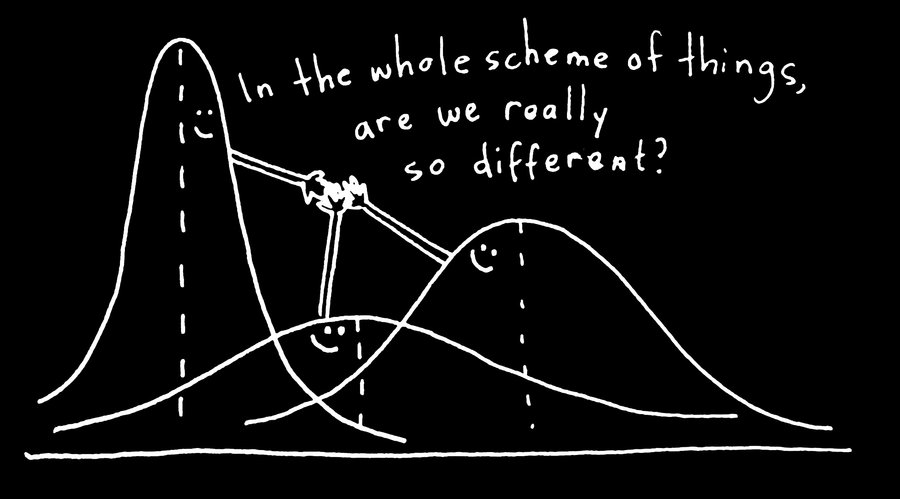
\includegraphics[scale=0.25]{ANOVA_Illustration-neg.png}
\end{frame}
%-------------- end slide -------------------------------%}}}
%-------------- start slide -------------------------------%{{{ 12.5
\begin{frame}

	\begin{enumerate}
		\item[E.g. 1] Study the relation between smoking and heart rates.\\[1em]
Generations of athletes have been cautioned that cigarette smoking impedes
performance. One measure of the truth of that warning is the effect of smoking
on heart rate. In one study, six nonsmokers, six light smokers, six moderate
smokers, and six heavy smokers each engaged in sustained physical exercise.
Table 8.1.1 lists their heart rates after they had rested for three minutes.
\\[1em]
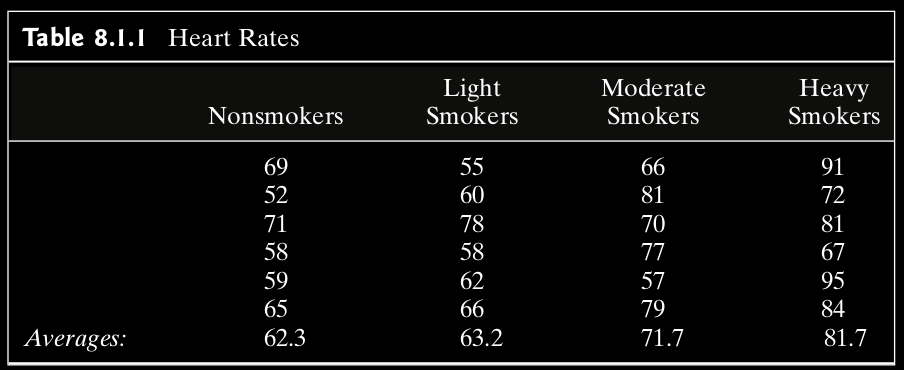
\includegraphics[scale=0.25]{Table_8-1-1-neg.png}
\item[] Show whether smoking affects heart rates at $\alpha=0.05$.
	\end{enumerate}
\end{frame}
%-------------- end slide -------------------------------%}}}
%-------------- start slide -------------------------------%{{{ 12.6
\begin{frame}
	\begin{enumerate}
		\item[E.g. 2] A certain fraction of antibiotics injected into the bloodstream are ``bound'' to
serum proteins. This phenomenon bears directly on the effectiveness of the
medication, because the binding decreases the systemic uptake of the drug.
Table below lists the binding percentages in bovine serum measured for five
widely prescribed antibiotics. Which antibiotics have similar binding
properties, and which are different? \\[1em]
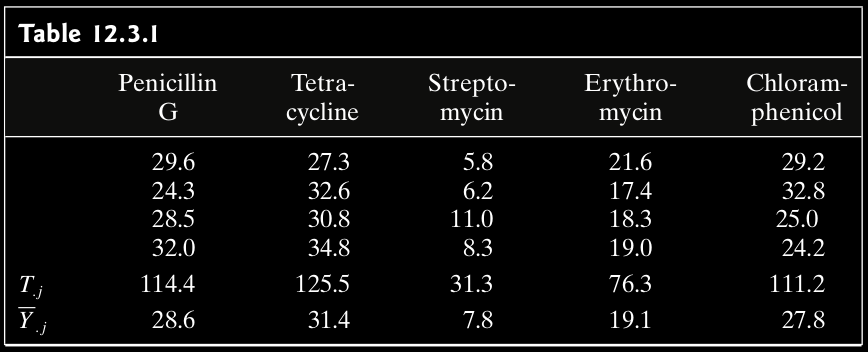
\includegraphics[scale=0.25]{Table_12-3-1-neg.png}
	\end{enumerate}
\end{frame}
%-------------- end slide -------------------------------%}}}
%-------------- start slide -------------------------------%{{{ 12.7
\begin{frame}
	\centering
	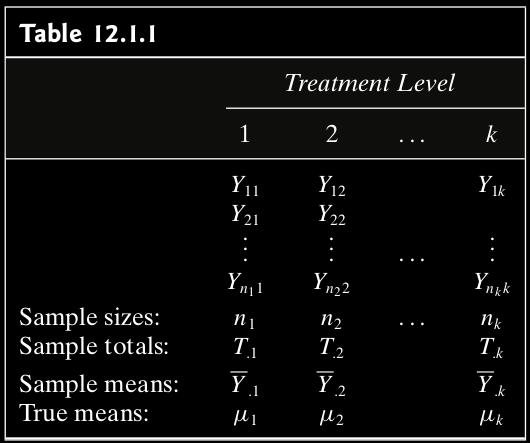
\includegraphics[scale=0.25]{Table_12-1-1-neg.png}
	\vfill
	\begin{itemize}
		\item $k$ treatment levels; $k$ independent random sample of size $n_1,\cdots, n_k$
			\vfill
		\item Total sample size: $n=\sum_{i=1}^k n_i$
			\vfill
		\item $Y_{ij}$: $i$-th observation for the $j$-th level.
			\vfill
		\item Sample total: $T_{\cdot j} = \sum_{i=1}^{n_j}Y_{i j}$
			\vfill
		\item Sample mean: $\overline{Y}_{\cdot j} = \frac{1}{n_j}\sum_{i=1}^{n_j}Y_{i j} = \frac{T_{\cdot j}}{n_j}$
			\vfill
		\item Overall total: $T_{\cdot \cdot} = \sum_{j=1}^k \sum_{i=1}^{n_j}Y_{i j}=\sum_{j=1}^k T_{\cdot j}$
			\vfill
		\item Overall mean: $\overline{Y}_{\cdot \cdot} =\frac{1}{n}\sum_{j=1}^k \sum_{i=1}^{n_j}Y_{i j} = \frac{1}{n}\sum_{j=1}^k n_j \overline{Y}_{\cdot j} = \frac{1}{n}\sum_{j=1}^k T_{\cdot j}$
	\end{itemize}
\end{frame}
%-------------- end slide -------------------------------%}}}
%-------------- start slide -------------------------------%{{{ 12.8
\begin{frame}

	\begin{enumerate}
		\item[Assume] For $j=1,\cdots, k$, $Y_{ij}\sim N(\mu_j,\sigma_j^2)$ and $\sigma_1^2 = \cdots =\sigma_k^2 = \sigma^2$ (unknown).
			\vfill
		\item[Problem] Testing
			\begin{gather*}
				H_0 : \mu_1=\mu_2=\cdots = \mu_k\\
				      \text{versus}\\
				H_1: \text{not all the $\mu_j$'s are equal}
			\end{gather*}
			\vfill
		\item[] Or testing \textcolor{yellow!80!black}{\it subhypotheses} such as\\[2em]
			\[
				H_0 : \mu_i = \mu_j \quad\text{or}\quad
				H_0 : \mu_3 = (\mu_1+\mu_2)/2
			\]
	\end{enumerate}
\end{frame}
%-------------- end slide -------------------------------%}}}
%-------------- start slide -------------------------------%{{{ 12.9
\begin{frame}
\centering
ANOVA was developed by statistician and evolutionary biologist ---
\vfill
% 
\includegraphics[scale=0.17]{Fisher.png}
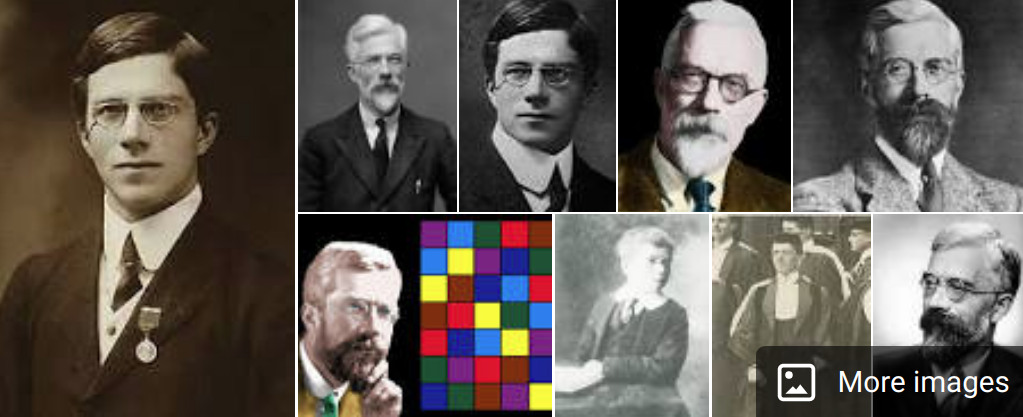
\includegraphics[scale=0.17]{Fisher-Portrait.png}

\includegraphics[scale=0.17]{Fisher-Intro-neg.png}
\end{frame}
%-------------- end slide -------------------------------%}}}
%-------------- start slide -------------------------------%{{{ 12.10
\begin{frame}[fragile]
	\begin{center}
		\url{https://www.youtube.com/watch?v=0XsovsSnRuw}
	\end{center}
\end{frame}
%-------------- end slide -------------------------------%}}}
